\section{Problem 1}
\subsection{Implementing PCA}

Below is my implementation of PCA, reusing the same PCA that I implemented in Assignment 3
It has been slightly modified to match this weeks dataset.
\begin{minted}[linenos, bgcolor = bg, breaklines]{python}
    def __PCA(data):
    
    # Creating "clone" of matrix
    data_cent = np.full_like(data,0) 
    # Iterate the matrix subtracting the mean from each row
    for i in range(4):
        data_cent[:,i] = trainingFeatures[:,i] - np.mean(trainingFeatures, 1)

    # Transposes the data
    data_cent = data_cent.T
    # Creates Covariance matrix for data_cent
    cov2 = np.cov(data_cent)
    # Calculates eigenvalues and eigenvectors
    PCevals, PCevecs = np.linalg.eig(cov2)

    return PCevals, PCevecs
\end{minted}

% \begin{figure}[H]
%     \centering
%     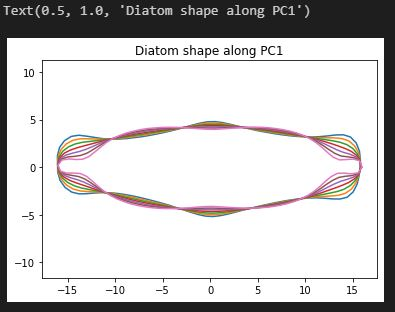
\includegraphics[width=0.75\textwidth]{Figures/Result_of_diatoms.JPG}
%     \caption{Plotted diatom}
% \end{figure}

\newpage